\documentclass[12pt]{article}

\usepackage[T1]{fontenc}
\usepackage[utf8]{inputenc}
\usepackage[italian]{babel}
\usepackage{fancyhdr}
\usepackage[margin=2cm]{geometry}
\usepackage{tocloft}
\usepackage{amsmath}
\usepackage{enumitem}
\usepackage{rotating}
\usepackage{graphicx}
\usepackage{hyperref}

\renewcommand{\cftsecleader}{\cftdotfill{\cftdotsep}}
\renewcommand{\thesection}{\arabic{section}.}
\renewcommand{\thesubsection}{\arabic{section}.\arabic{subsection}}

\setlength{\headheight}{15pt}

\pagestyle{fancy}
\renewcommand{\footrulewidth}{0.4pt}
\lhead{\bfseries Requisiti di sistema}
\chead{}
\rhead{}
\lfoot{}
\cfoot{}
\rfoot{\thepage}


\usepackage{titlesec}
\usepackage{hyperref}
\titleclass{\subsubsubsection}{straight}[\subsection]

\newcounter{subsubsubsection}[subsubsection]
\renewcommand\thesubsubsubsection{\thesubsubsection.\arabic{subsubsubsection}}
\renewcommand\theparagraph{\thesubsubsubsection.\arabic{paragraph}} % optional; useful if paragraphs are to be numbered

\titleformat{\subsubsubsection}
  {\normalfont\normalsize\bfseries}{\thesubsubsubsection}{1em}{}
\titlespacing*{\subsubsubsection}
{0pt}{3.25ex plus 1ex minus .2ex}{1.5ex plus .2ex}

\makeatletter
\renewcommand\paragraph{\@startsection{paragraph}{5}{\z@}%
  {3.25ex \@plus1ex \@minus.2ex}%
  {-1em}%
  {\normalfont\normalsize\bfseries}}
\renewcommand\subparagraph{\@startsection{subparagraph}{6}{\parindent}%
  {3.25ex \@plus1ex \@minus .2ex}%
  {-1em}%
  {\normalfont\normalsize\bfseries}}
\def\toclevel@subsubsubsection{4}
\def\toclevel@paragraph{5}
\def\toclevel@paragraph{6}
\def\l@subsubsubsection{\@dottedtocline{4}{7em}{4em}}
\def\l@paragraph{\@dottedtocline{5}{10em}{5em}}
\def\l@subparagraph{\@dottedtocline{6}{14em}{6em}}
\makeatother

\setcounter{secnumdepth}{4}
\setcounter{tocdepth}{4}



\begin{document}
\tableofcontents

\pagebreak

\section{Prefazione}

\subsection{Version History}

Versione 0.0 - 16/04/2019

\subsection{Sommario modifiche}
Definizione dei requisiti funzionali, dei casi d'uso, della struttura generale del software, della struttura dei test e degli strumenti utilizzati per lo sviluppo.

\pagebreak

\section{Introduction}

\subsection{Definizioni e glossario}
\subsubsection*{Grammatica libera da contesto}
In informatica e in linguistica, una grammatica libera dal contesto è una grammatica formale in cui
ogni regola sintattica è espressa sotto forma di derivazione di un simbolo a sinistra a partire da uno
o più simboli a destra. \par
Ciò può essere espresso con due simbolismi equivalenti:
\begin{enumerate}[label=\arabic*)]
\item $S := \alpha$
\item $S \to \alpha$
\end{enumerate}
dove $S$ è un simbolo detto \textit{non terminale}, sostituibile con altri simboli non terminali e/o con simboli terminali, e $\alpha$ è una sequenza di simboli non terminali e/o terminali, ossia simboli che non possono essere sostituiti con null'altro. \par
L'espressione "libera dal contesto" si riferisce al fatto che il simbolo non terminale $S$ può sempre
essere sostituito da $\alpha$, indipendentemente dai simboli che lo precedono o lo seguono; un linguaggio
formale si dice libero dal contesto se esiste una grammatica libera dal contesto che lo genera.
\subsubsection*{Parser}
Un parser LR è un parser di tipo bottom-up per grammatiche libere da contesto che legge il proprio input partendo da sinistra verso destra, producendo una derivazione a destra. Laddove indicato come parser $LR \left( k \right)$, il $k$ si riferisce al numero di simboli letti (ma non "consumati") per prendere le decisioni di parsing.

\subsection{Scopo}
Scopo del programma che si andrà a realizzare è il riconoscimento di una grammatica LR(1) contenuta in un file di input selezionato dall'utente. \par

\pagebreak

\subsection{Toolchain}
Per lo sviluppo di questo progetto è stata scelta la seguente toolchain:
\begin{itemize}
\item Git, utilizzato per il controllo di versione, così da consentire il lavoro a più mani sul progetto anche qualora non ci si trovi tutti nello stesso ambiente. L'utilizzo di Git prevederà la creazione di branch secondari per gli sviluppi incrementali del programma, così da conservare sempre una versione funzionante del programma stesso all'interno del branch "master" della repository ospitante il progetto;
\item GitKraken, client che fornisce un'interfaccia grafica intuitiva per l'utilizzo di github, implementa funzioni che velocizzano l'utilizzo di git implementando un grafo rappresentante l'avanzamento della repository.
\item Modelio, utilizzato per la creazione di diagrammi UML, si è scelto questo tool visto che implementa dei tool che partendo da codice java genera il modello UML del codice fornito. Essendo questo progetto un'espansione di un progetto già in essere realizzato per il corso Linguaggi Formali e Compilatori questo tool agevolerà la creazione del modello UML del codice già esistente;
\item TexMaker, utilizzato per la redazione della documentazione;
\item Eclipse, utilizzato per lo sviluppo dell'applicazione, inoltre integra dei tool utili al fine di analizzare la copertura del codice;
\item ANTLR, tool per la generazione di parser, una volta definita una grammatica questo genera un parser e tutto il codice di contorno per l'individuazione di errori lessicali e semantici;
\item Junit, tool utilizzato per la definizione dei casi di test e l'esecuzione dei casi stessi;
\item SpotBugs, PMD, plugin di Eclipse utilizzati per l'analisi statica del codice.
\end{itemize}

\pagebreak

\section{Iterazione 0}

\subsection{Requisiti funzionali}
Il programma deve consentire all'utente le seguenti azioni:
\begin{itemize}
\item selezione del file di input da sottoporre al parsing e all'identificazione.
\end{itemize}
Il programma deve fornire le seguenti funzionalità:
\begin{itemize}
\item effettuare il parsing del file ricevuto in input, individuando eventuali errori sintattici, lessicali o semantici;
\item qualora vengano individuati errori di qualsiasi genere nella fase di parsing, il programma deve comunicare i dettagli relativi agli errori individuati all'utente;
\item qualora non vengano individuati errori nella fase di parsing, il programma deve procedere nell'identificare la grammatica come grammatica $LR \left( 1 \right)$ o non $LR \left( 1 \right)$.
\end{itemize}  

\subsubsection{Struttura corretta della grammatica}\label{struttura}
Il programma deve riconoscere come formalmente corrette (quindi prive di errori sintattici, lessicali e/o grammaticali) soltanto grammatiche che presentino la seguente struttura:
\begin{itemize}
\item una prima regola $pr$ che abbia come elemento di sinistra il non terminale $S0$, definita come segue
$$
SZ \hspace{5pt} EQ \hspace{5pt} NT \hspace{5pt} TER \hspace{5pt} SC
$$
\item altre $n \geq 1$ regole di produzione $ar$, che formano il resto della grammatica, definite come segue
$$
NT \hspace{5pt} EQ \hspace{5pt} \left( NT \left| CT \right. \right)^* \hspace{5pt} SC
$$
\end{itemize}
I blocchi componenti le regole appena definite sono così traducibili:
\begin{table}[h]
\centering
\begin{tabular}{|c|c|}
\hline
\textbf{Simbolo} & \textbf{Caratteri} \\
\hline
$SZ$ & $S0$ \\
\hline
$EQ$ & $-> \left| \hspace{5pt} := \right.$ \\
\hline
$NT$ & $A \hspace{5pt} \dots \hspace{5pt} Z$ \\
\hline
$CT$ & $a \hspace{3pt} \dots z \left| \hspace{3pt} 0 \hspace{3pt} \dots \hspace{3pt} 9 \hspace{3pt} \right| \hspace{3pt} + \hspace{3pt} \left| \hspace{3pt} - \hspace{3pt} \right| \hspace{3pt} * \hspace{3pt} \left| \hspace{3pt} / \right.$ \\
\hline
$TER$ & $\text{/swa} \hspace{5pt} \left| \hspace{5pt} \text{/cjswa} \right.$ \\
\hline
$SC$ & $;$ \\
\hline
\end{tabular}
\caption{Corrispondenza tra caratteri della grammatica e blocchi di definizione delle regole}
\end{table}

\underline{Nota:} Per la definizione della struttura delle regole è stata utilizzata la notazione formale di Backus-Naur estesa (EBNF).

\subsubsection{Errori lessicali}
L'utilizzo di qualsiasi carattere non riconducibile alla colonna "Caratteri" della Tabella 1 corrisponde a un errore lessicale.

\subsubsection{Errori sintattici}
Gli errori sintattici sono dati dal mancato rispetto della struttura delle regole $pr$ e $ar$ come definite nel paragrafo "Struttura corretta della grammatica" a pagina \pageref{struttura}.

\subsubsection{Errori semantici}
Gli errori semantici si verificano nei seguenti casi:
\begin{itemize}
\item nella grammatica è presente un carattere non terminale che non presenta regole di produzioni associate;
\item nella grammatica è presente una regola duplicata (\underline{nota bene} questo \underline{non} è un errore bloccante).
\end{itemize}
\pagebreak

\subsection{Casi d'uso}
In questa fase preliminare si è identificato un solo caso d'uso riportato di seguito

\subsubsection{UC1 - Analisi di una grammatica}
\begin{itemize}[label=]
\item \textbf{Descrizione:} identificazione di una grammatica $LR\left( 1 \right)$
\item \textbf{Attori coinvolti:} utente
\item \textbf{Precondizioni:} esistenza del file d'input contenente la definizione della grammatica
\item \textbf{Trigger:} necessità di identificare una grammatica
\item \textbf{Post condizioni:} la classificazione della grammatica viene mostrata a schermo
\item \textbf{Procedimento standard:}
\begin{enumerate}[label=\arabic*.]
\item l'utente avvia il programma;
\item l'utente seleziona il file di input desiderato;
\item il programma esegue il parsing e l'analisi del file di input;
\item il programma mostra a schermo l'esito dell'analisi della grammatica;
\item l'utente chiude il programma.
\end{enumerate}
\textbf{Procedimenti alternativi o eccezioni:}
\begin{itemize}
\item allo step $3$, il programma rileva errori nella grammatica
\begin{itemize}[label=]
\item viene mostrato un messaggio d'errore contenente informazioni relative all'errore individuato, l'utente chiude il programma e, corretta la grammatica, la procedura riparte dallo step $1$
\end{itemize}
\end{itemize}
\end{itemize}
\pagebreak

\subsection{Struttura del programma}
Il programma, definito in linguaggio Java, sarà composto di tre moduli:
\begin{itemize}
\item un primo modulo che verrà implementato all'interno del modulo generato da ANTLR, che si occuperà della lettura di un file .txt contenente la grammatica da identificare.
\item un modulo generato da ANTLR, che si occuperà del parsing e dell'individuazione di errori lessicali e sintattici;
\item un modulo scritto manualmente che si occuperà dell'analisi della grammatica e della sua classificazione.
\end{itemize}
L'interfacciamento con l'utente nella priva versione avverrà attraverso una CLI (Command Line Interface).


\subsubsection{Scelta architetturale}\label{bozzaArc}
Vista la struttura del programma si è scelto la struttura ideale è di tipo pipe and filter dove si possono identificare specifici moduli e ogni modulo genera dei risultati intermedi che verranno poi utilizzati dai moduli successivi.\par
In figura è riportata una bozza della struttura implementata nella fase 1.
\par

\begin{figure}[h]
\centering
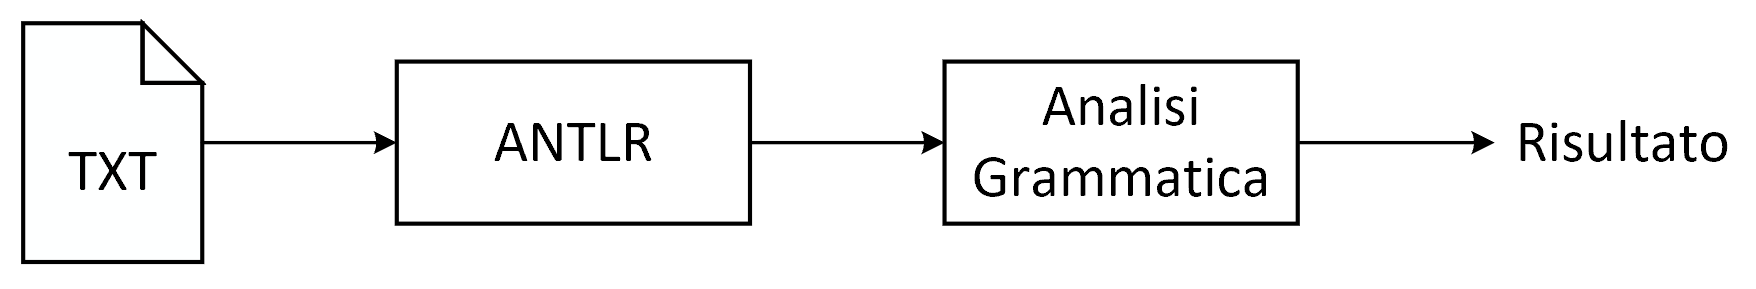
\includegraphics[scale=0.8]{immagini/bozzaArchitettura_v0.png}
\caption{Bozza dell'architettura}
\end{figure}

\pagebreak

\subsection{Programma di testing}
Il testing del programma sarà incentrato sul modulo \textit{non} generato da ANTLR, assumendo che i controlli su quello generato da ANTLR siano già stati svolti dal produttore del tool, e sarà composto di:
\begin{itemize}
\item casi di test per ogni classe generata scritti in JUnit, per i quali sarà richiesta una coverage del codice $\geq 95\%$;
\item verifiche di coverage del codice scritto tramite l'esecuzione del programma con diversi input, al fine di garantire l'assenza di dead code;
\item analisi statica del codice tramite strumenti quali SpotBugs e PMD.
\end{itemize}
A ogni revisione del codice, nonché in precedenza al rilascio di una nuova versione, saranno svolti test di non regressione per evitare l'introduzione di nuovi difetti nel codice.
\pagebreak

\section{Iterazione 1}
In questa iterazione è stata creata la versione a CLI (Command Line Interface), è stata inserita un'unica interfaccia grafica utilizzata per permettere all'utente la selezione del file che contiene la grammatica da analizzare, l'esito dell'analisi è riportato all'interno della CLI indicando se la grammatica è o meno LR(1), l'elenco di tutti gli stati ed infine un elenco di tutte le transizioni.
\subsection{Design Architetturale}
In questa prima versione il design architetturale è rimasto quello previsto nella iterazione 0.
\subsubsection{Class diagram}
Per la generazione del class diagram della fase 1 è stato utilizzato il tool "java designer" di Modelio che premette di estrapolare dal codice già presente il diagramma UML delle classi.
In particolare si può notare come la struttura sequenziale del programma è molto simile a quella ipotizzata nella fase zero a pagina \pageref{bozzaArc}.

\begin{sidewaysfigure}\label{rifUMLV1}
\centering
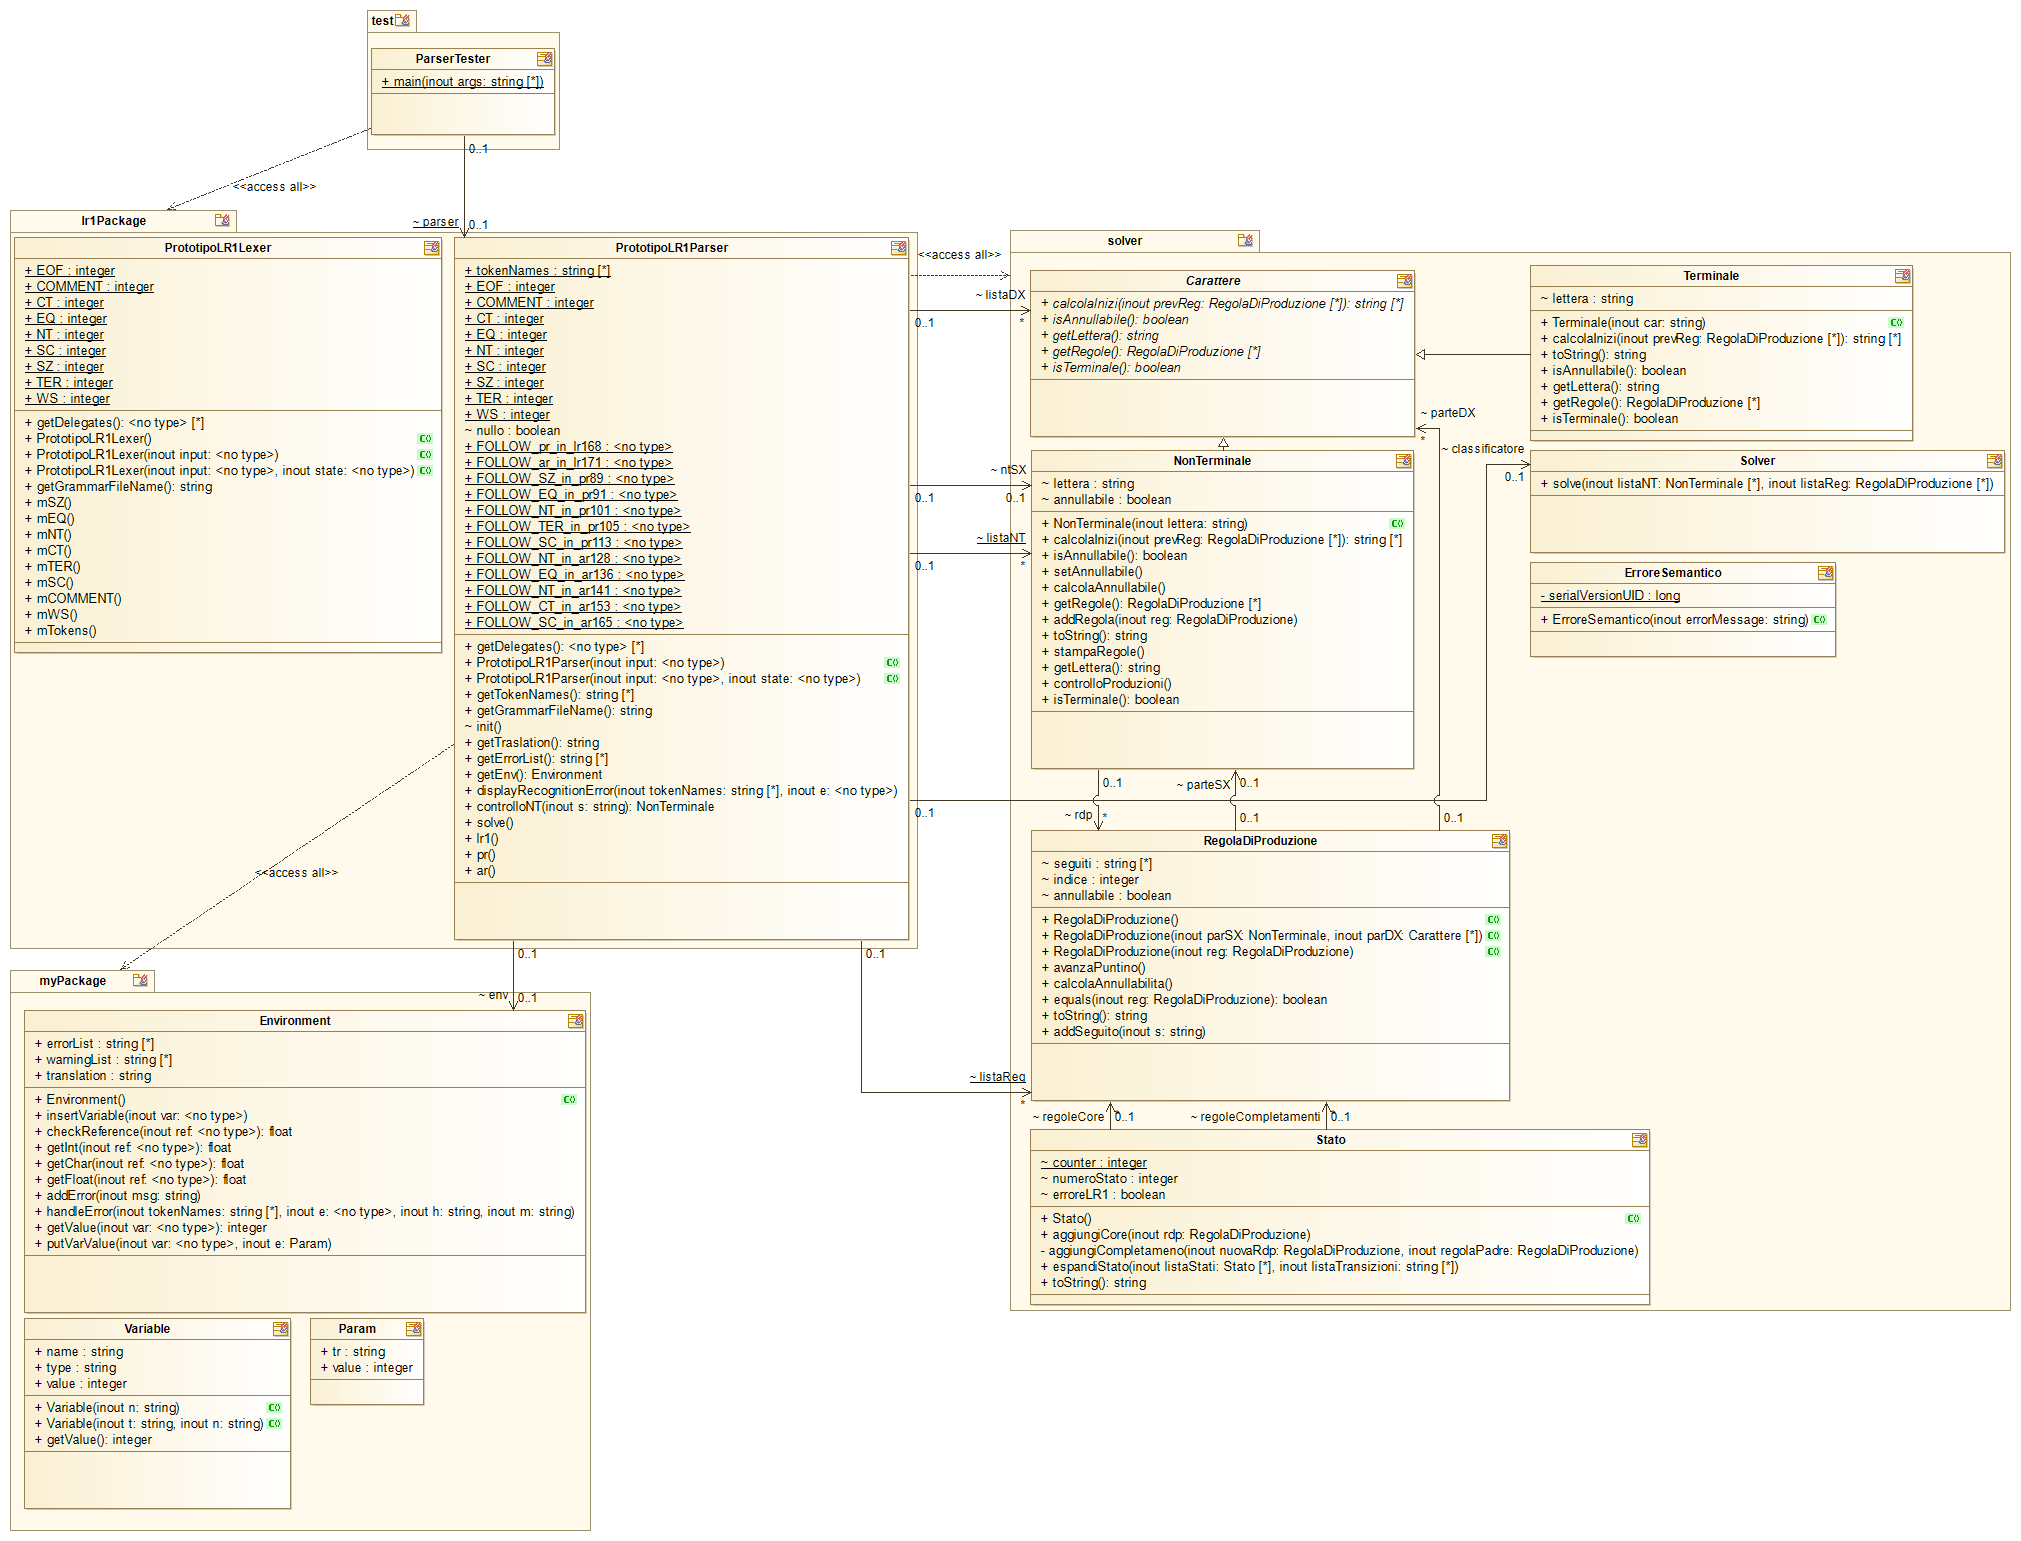
\includegraphics[scale=0.4]{immagini/UMLV1.png}
\caption{UML Class Diagram delle funzionalità dell'applicazione nell'iterazione 1}
\end{sidewaysfigure}
\pagebreak

\subsection{Testing}
\subsubsection{Descrizione del prodotto software}
Il software, sviluppato in linguaggio Java in ambiente di sviluppo Eclipse, è suddiviso nei $4$ packages descritti di seguito:
\begin{itemize}
\item \textbf{lr1package} - questo package contiene due degli output di ANTLR, strumento utilizzato per generare il compilatore, ossia \textit{PrototipoLR1Lexer.java} e \textit{PrototipoLR1Parser.java}; il terzo e ultimo file di output (\textit{PrototipoLR1.tokens} è invece situato all'esterno di questo package;
\item \textbf{main\_package} - questo package contiene il file \textit{Riconoscitore.java}, all'interno del quale è definito il metodo \textit{main} che permette l'effettiva esecuzione del programma;
\item \textbf{myPackage} - questo package contiene il file \textit{Environment.java}, all'interno del quale è definita la classe Environment, necessaria per il corretto funzionamento dei file output di ANTLR ed ereditata da un progetto di esempio;
\item \textbf{solver} - questo package contiene tutti i file che contengono definizioni di classi custom utilizzate per il processo di riconoscimento delle grammatiche e per rappresentare gli elementi costituenti delle grammatiche.
\end{itemize}
La versione oggetto di test è la 1.0, pubblicata sul branch \textit{master} della repository di Github del progetto (\url{https://github.com/d-presciani/progettoLFC}) in data 26/03/2019.
\pagebreak

\subsubsection{Funzionalità oggetto di test}
Le funzionalità sottoposte a test di unità saranno quelle definite nelle classi contenute all'interno del package \textit{solver}, essendo queste le classi scritte manualmente e quelle che consentono l'effettivo funzionamento del programma; si tralascia di effettuare test di unità sui restanti package in quanto generati automaticamente da ANTLR e difficilmente sottoponibili a test di tale granularità. \par
È previsto anche un test di sistema, fornendo al sistema diversi input, per verificare la corretta integrazione tra i vari componenti e, al contempo, il corretto funzionamento del programma nel suo complesso. \par
Oltre ai suddetti test, è prevista anche l'esecuzione di un'analisi statica del codice tramite i due plugin di Eclipse \textit{SpotBugs} e \textit{PMD}.
\subsubsubsection{Elenco delle funzionalità oggetto di test}
Di seguito vengono riportate le classi, con i relativi metodi, per cui saranno effettuati i test di unità.
\begin{itemize}
\item Stato
\begin{itemize}
\item private void aggiungiCompletamento(RegolaDiProduzione nuovaRdp, RegolaDiProduzione regolaPadre)
\item public void aggiungiCore(RegolaDiProduzione rdp)
\item public Stato()
\item public void espandiStato(LinkedList<Stato> listaStati, LinkedList<String> listaTransizioni)
\item public String toString()
\end{itemize}
\item RegolaDiProduzione
\begin{itemize}
\item public RegolaDiProduzione()
\item public RegolaDiProduzione(NonTerminale parSX, List<Carattere> parDX)
\item public RegolaDiProduzione(RegolaDiProduzione reg)
\item public void addSeguito(String s)
\item public void avanzaPuntino()
\item public void calcolaAnnullabilita()
\item public boolean equals(Object o)
\item public String toString()
\end{itemize}
\item NonTerminale
\begin{itemize}
\item public NonTerminale (String lettera)
\item public void addRegola (RegolaDiProduzione reg)
\item public void calcolaAnnullabile()
\item public List<String> calcolaInizi(LinkedList<RegolaDiProduzione> prevReg)
\item public void controlloProduzioni()
\item public String getLettera()
\item public List<RegolaDiProduzione> getRegole()
\item public boolean isAnnullabile()
\item public boolean isTerminale()
\item public void setAnnullabile()
\item public void stampaRegole()
\item public String toString()
\end{itemize}
\item Solver
\begin{itemize}
\item public boolean solve(LinkedList<NonTerminale> listaNT, \\
\hspace*{104pt} LinkedList<RegolaDiProduzione> listaReg)
\end{itemize}
\item Terminale
\begin{itemize}
\item public Terminale(String car)
\item public List<String> calcolaInizi(LinkedList<RegolaDiProduzione> prevReg)
\item public String getLettera()
\item public List<RegolaDiProduzione> getRegole()
\item public boolean isAnnullabile()
\item public boolean isTerminale()
\item public String toString()
\end{itemize}
\end{itemize}
\pagebreak

\subsection{Esiti dei test}
\subsubsection{Esiti e copertura dei test di unità}
Di seguito sono riportati gli esiti dei test e la copertura degli stessi per ognuna delle classe precedentemente evidenziate come oggetto di test di unità; nel complesso tali test hanno consentito una copertura del package \textit{solver} pari al $96,4\%$.
\begin{figure}[h]
\centering
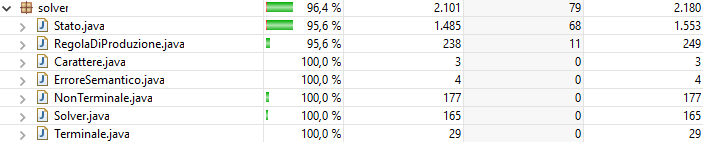
\includegraphics[width=\textwidth]{immagini/V1SolverCoverage.png}
\caption{Copertura dei test per il package solver}
\end{figure}
\subsubsubsection{Esiti dei test per la classe Stato}
Per la classe Stato sono stati scritti, all'interno della classe StatoTest, 22 test, superati correttamente dal programma, che garantiscono una copertura della classe Stato pari al $95,6\%$.
\begin{figure}[h]
\centering
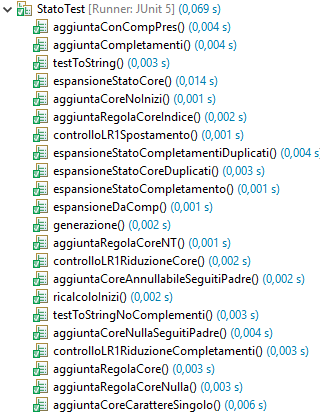
\includegraphics[scale=0.9]{immagini/V1esitiStatoTest.png}
\caption{Esiti dei test della classe Stato}
\end{figure}
\subsubsubsection{Esiti dei test per la classe RegolaDiProduzione}
Per la classe RegolaDiProduzione sono stati scritti, all'interno della classe RegolaDiProduzioneTest, 6 test, superati correttamente dal programma, che garantiscono una copertura della classe RegolaDiProduzione pari al $95,6\%$.
\begin{figure}[h]
\centering
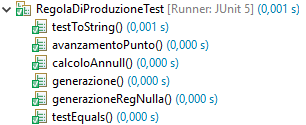
\includegraphics[scale=0.9]{immagini/V1esitiRegolaDiProduzioneTest.png}
\caption{Esiti dei test della classe RegolaDiProduzione}
\end{figure}
\subsubsubsection{Esiti dei test per la classe NonTerminale}
Per la classe NonTerminale sono stati scritti, all'interno della classe NonTerminaleTest, 13 test, superati correttamente dal programma, che garantiscono una copertura della classe NonTerminale pari al $100,0\%$.
\begin{figure}[h]
\centering
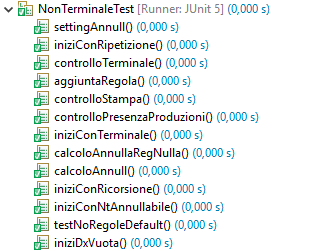
\includegraphics[scale=0.9]{immagini/V1esitiNonTerminaleTest.png}
\caption{Esiti dei test della classe NonTerminale}
\end{figure}
\pagebreak
\subsubsubsection{Esiti dei test per la classe Solver}
Per la classe Solver sono stati scritti, all'interno della classe SolverTest, 2 test, superati correttamente dal programma, che garantiscono una copertura della classe Solver pari al $100,0\%$.
\begin{figure}[h]
\centering
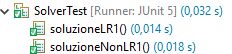
\includegraphics[scale=0.9]{immagini/V1esitiSolverTest.png}
\caption{Esiti dei test della classe Solver}
\end{figure}
\subsubsubsection{Esiti dei test per la classe Terminale}
Per la classe Terminale sono stati scritti, all'interno della classe TerminaleTest, 7 test, superati correttamente dal programma, che garantiscono una copertura della classe Terminale pari al $100,0\%$.
\begin{figure}[h]
\centering
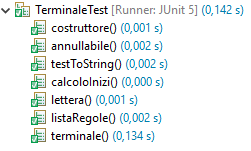
\includegraphics[scale=0.9]{immagini/V1esitiTerminaleTest.png}
\caption{Esiti dei test della classe Terminale}
\end{figure}
\pagebreak

\subsubsection{Esiti e copertura dei test di sistema}
I test di sistema sono stati effettuati eseguendo il metodo \textit{main} della classe \textit{Riconoscitore} più volte, passandogli come input i file contenuti all'interno della cartella "lfc$\backslash$resourses" presente nella repository del progetto (\url{https://github.com/d-presciani/progettoLFC}); come oracoli per valutare la correttezza dei test sono stati utilizzati i temi svolti in classe durante il corso di Linguaggi formali e compilatori. \par
Durante i test di sistema è stata rilevata anche la copertura del codice nelle varie esecuzioni; nella seguente immagine è possibile vedere la copertura complessiva (ottenuta combinando la copertura delle singole esecuzioni).
\begin{figure}[h]
\centering
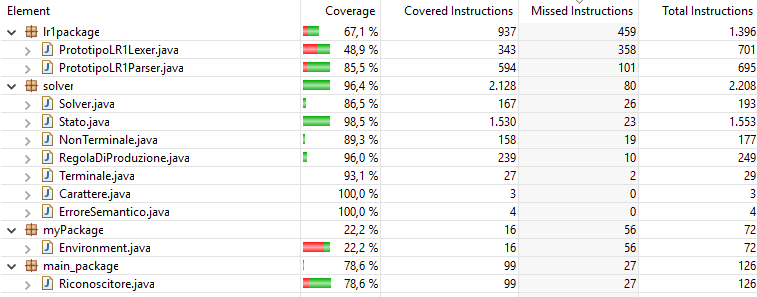
\includegraphics[width=\textwidth]{immagini/V1codeCoverage.png}
\caption{Copertura del codice relativa ai test di sistema}
\end{figure}
\pagebreak

\section{Iterazione 2}
In questa iterazione è stata implementata un interfaccia grafica che permette di interagire con il programma in un ambiente completamente grafico.\par
È stata aggiunta inoltre la possibilità di visualizzare graficamente il risultato dell'analisi generando un grafo della grammatica analizzata.
\subsection{Design Architetturale}
In questa seconda versione la struttura è rimasta di tipo pipe and filter ma è stata ampliata per includere la generazione e la visualizzazione del grafo, come si può vedere in figura.
\begin{figure}[h]
\centering
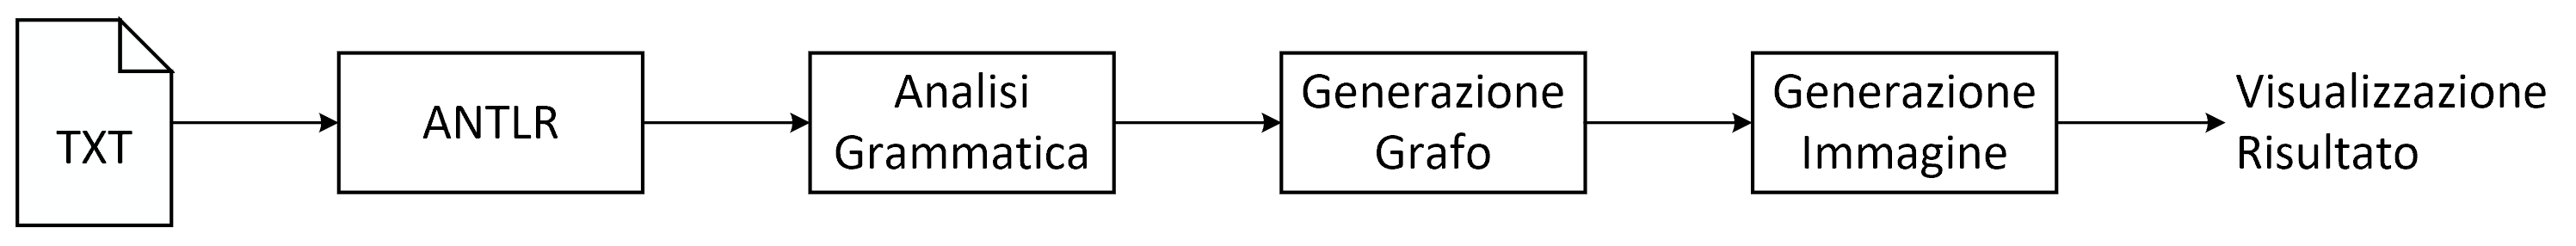
\includegraphics[width=\textwidth]{immagini/bozzaArchitettura_v2.png}
\caption{Bozza dell'architettura nella seconda iterazione}
\end{figure}
\pagebreak
\subsubsection{Librerie utilizzate}
Per l'implementazione dell'interfaccia grafica e la creazione del grafo sono state utilizzate le seguenti librerie:
\begin{itemize}
\item JavaFX, framework grafico utilizzato per la realizzazione dell'interfaccia utente;
\item JgraphT, libreria realizzata in swing che permette la creazione di grafi di vario tipo, implementando inoltre iteratori può essere utilizzata per la creazione di algoritmi di vario tipo;
\item mxGraph, libreria che permette la creazione di diagrammi e utilizza SVG e HTML per il rendering delle immagini, in questo progetto questa libreria è utilizzata per la visualizzazione del grafico creato con JgraphT, in particolare questa libreria è stata scelta perché permette se integrata in un Jframe di modificare l'aspetto del grafico in realtime oltre che offrire molte opzioni per la personalizzazione dei grafici.
Nella pratica questa libreria è stata utilizzata per modificare l'aspetto delle box cambiando colore agli stati che contengono delle regole che rendono il linguaggio non LR(1) e per modificare lo stile grafico di rappresentazione.
\end{itemize}

Durante lo sviluppo di questa iterazione sono però sorte delle problematiche nell'integrazione delle librerie per la generazione del grafo e JavaFx.\par
Provando ad integrare all'interno dell'interfaccia utente un modulo sviluppato per testare le funzionalità di mxGraph che implementava la modifica realtime del grafo, sono stati riscontrati alcuni problemi di integrabilità essendo questa libreria realizzata in swing.\par
Per implementare questo modulo si è provato ad utilizzare la classe SwingNode per "incaplsulare" questo modulo che integra componenti realizzate in swing e riuscire quindi a riutilizzare correttamente il modulo all'interno dell'interfaccia utente creata con JavaFX.\par
Dopo diversi tentativi si è riusciti ad integrare il modulo contenente il grafo con l'interfaccia utente realizzata con JavaFX, perdendo però la possibilità di editare in tempo reale il grafico, si è dunque scelto per motivi di performance di salvare l'immagine generata tramite mxGraph (la scelta del formato è lasciata all'utente) e poi caricare l'immagine salvata all'interno dell'interfaccia grafica per la visualizzazione del grafo.

\subsubsection{Class Diagram}
Rispetto al class diagram presente a pagina \pageref{rifUMLV1} in questa nuova iterazione si può vedere come è stato necessario modificare la struttura delle classi per permettere il trasferimento di informazioni tra le classi in modo da poter mostrare all'interno dell'interfaccia grafica i vari messaggi da mostrare all'utente.

\begin{sidewaysfigure}
\centering
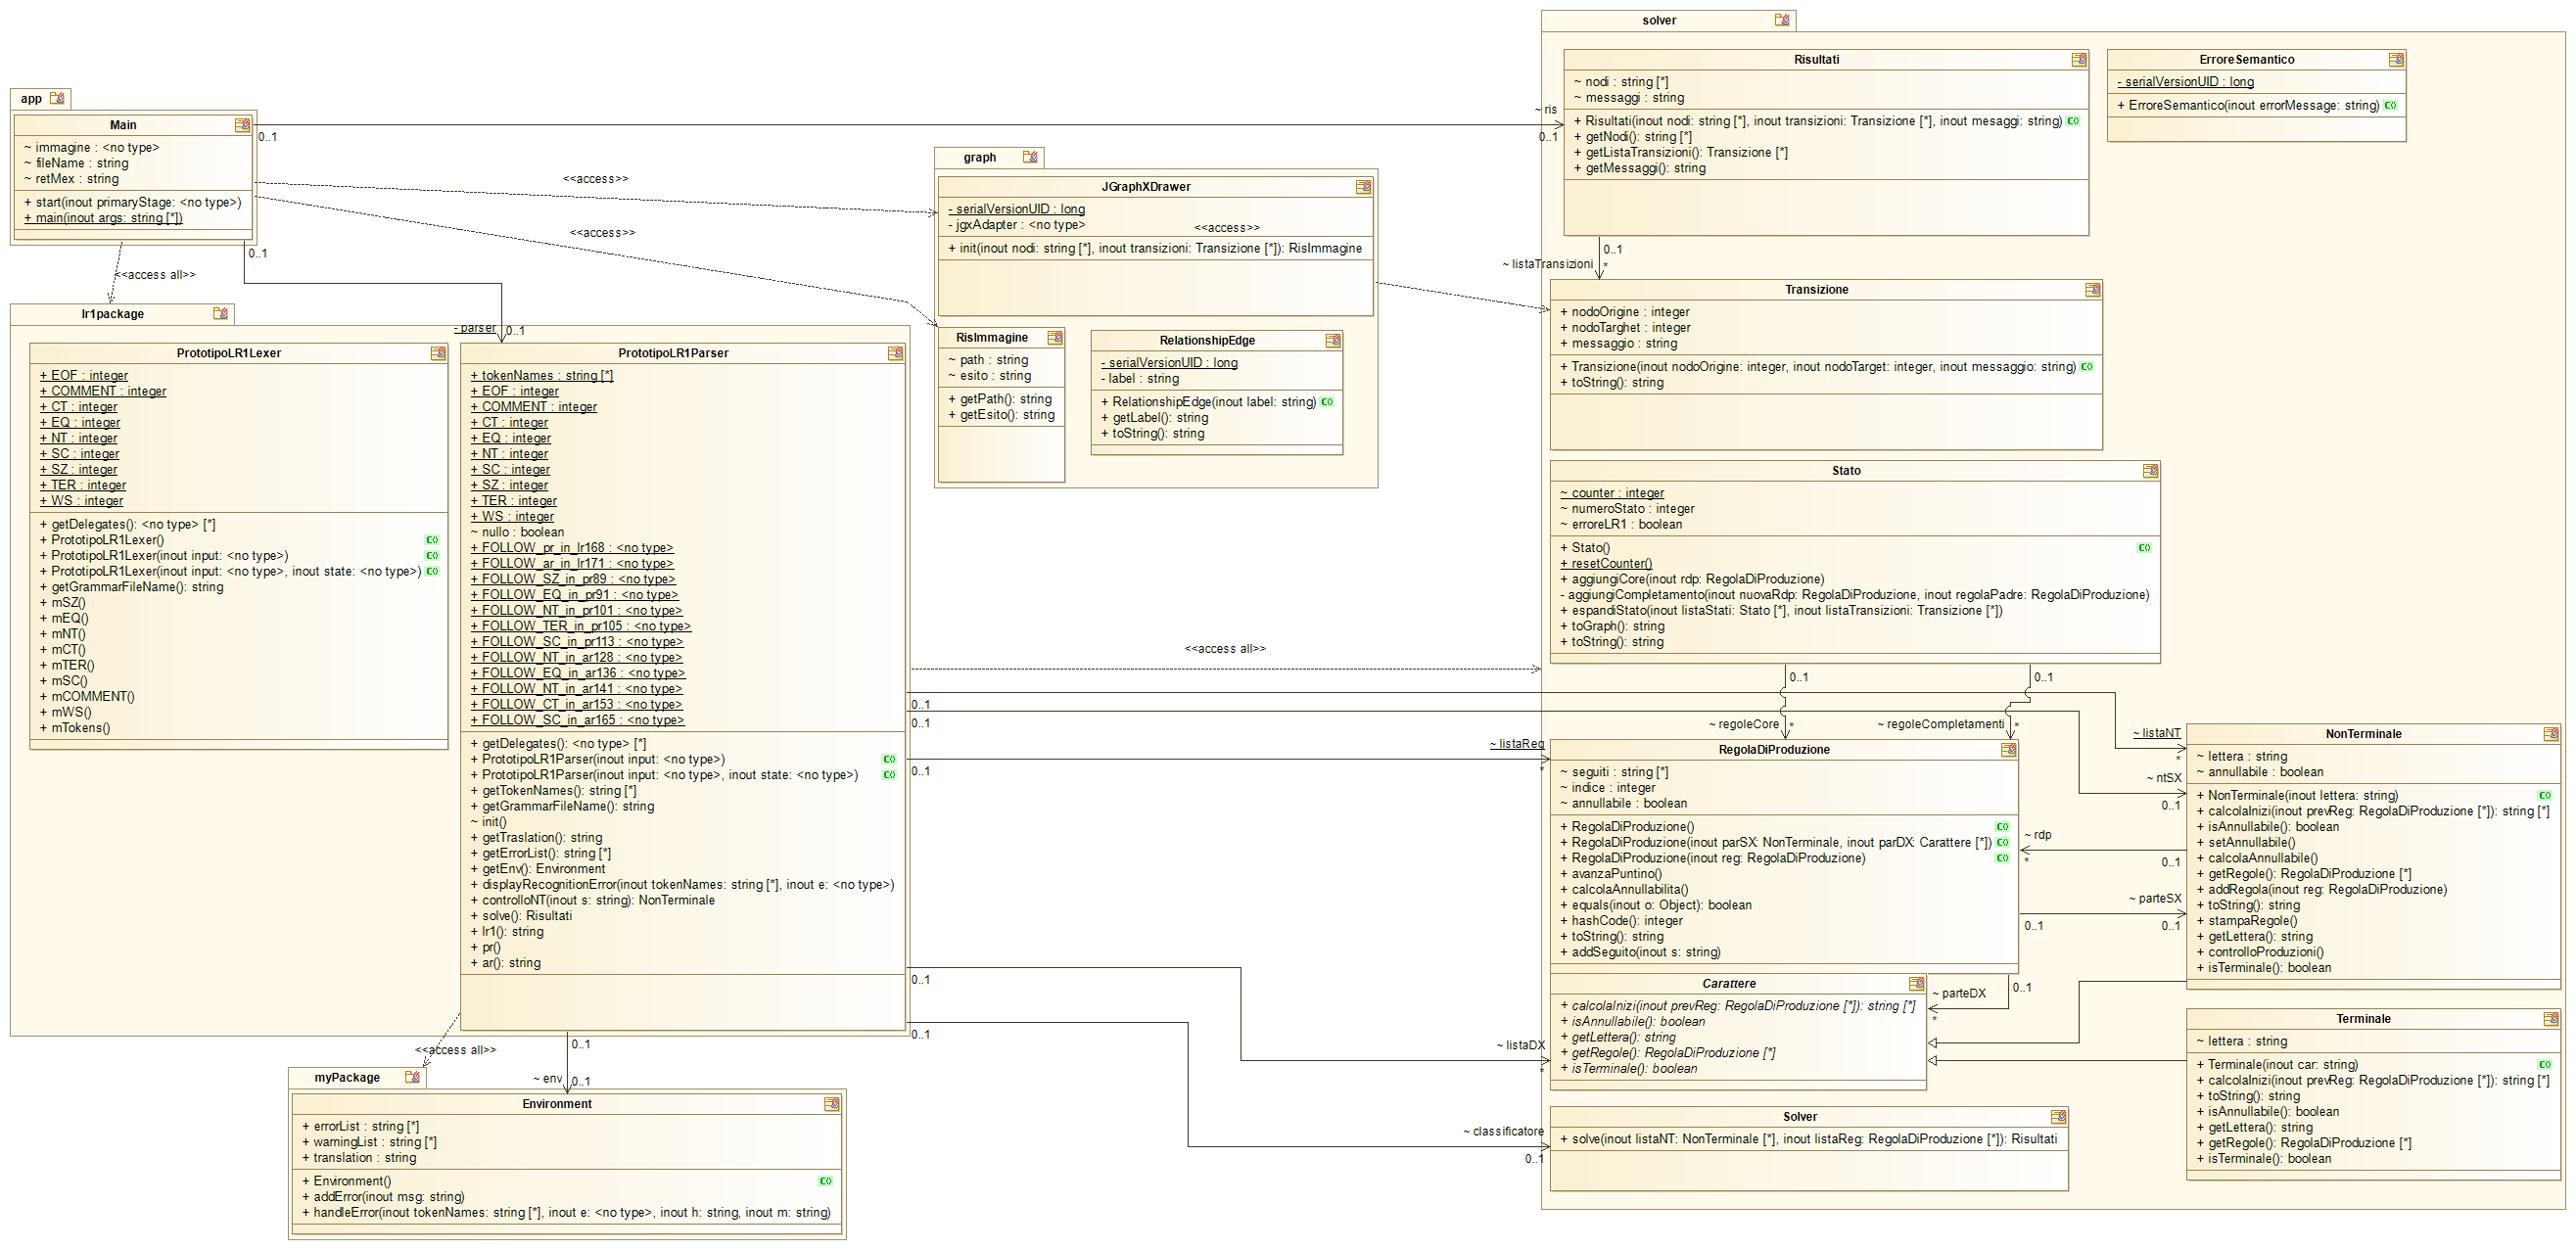
\includegraphics[scale=0.3]{immagini/UMLV2.png}
\caption{UML Class Diagram delle funzionalità dell'applicazione nell'iterazione 2}
\end{sidewaysfigure}
\pagebreak

\pagebreak
\subsection{Casi d'uso}
Vista l'introduzione di un'interfaccia grafica per l'interazione con il programma sono stati ridefiniti i casi d'uso come segue:
\subsubsection{UC1 - Analisi di una grammatica}
\begin{itemize}[label=]
\item \textbf{Descrizione:} identificazione di una grammatica $LR\left( 1 \right)$
\item \textbf{Attori coinvolti:} utente
\item \textbf{Precondizioni:} esistenza del file d'input contenente la definizione della grammatica
\item \textbf{Trigger:} necessità di identificare una grammatica
\item \textbf{Post condizioni:} la classificazione della grammatica viene mostrata a schermo
\item \textbf{Procedimento standard:}
\begin{enumerate}[label=\arabic*.]
\item l'utente avvia il programma;
\item l'utente clicca il pulsante "carica file";
\item l'utente seleziona il file di input desiderato;
\item il programma esegue il parsing e l'analisi del file di input;
\item il programma mostra a schermo l'esito dell'analisi della grammatica.
\end{enumerate}
\textbf{Procedimenti alternativi o eccezioni:}
\begin{itemize}
\item allo step $3$, il programma rileva errori nella grammatica
\begin{itemize}[label=]
\item viene mostrato un messaggio d'errore contenente informazioni relative all'errore individuato, l'utente, corretta la grammatica riprende la procedura dallo step $2$
\end{itemize}
\end{itemize}
\end{itemize}

\subsubsection{UC2 - Visualizzazione della grammatica analizzata}
\begin{itemize}[label=]
\item \textbf{Descrizione:} visualizzazione della grammatica $LR\left( 1 \right)$ analizzata precedentemente
\item \textbf{Attori coinvolti:} utente
\item \textbf{Precondizioni:} analisi di una grammatica avvenuta correttamente
\item \textbf{Trigger:} necessità di visualizzare la grammatica identificata
\item \textbf{Post condizioni:} creazione di un file contenente il grafo relativo alla grammatica e visualizzazione dello stesso
\item \textbf{Procedimento standard:}
\begin{enumerate}[label=\arabic*.]
\item l'utente clicca il pulsante "genera e mostra grafo";
\item l'utente seleziona la posizione dove salvare il grafo e il formato del file creato;
\item il programma genera e mostra a schermo il grafo relativo alla grammatica.
\end{enumerate}
\textbf{Procedimenti alternativi o eccezioni:}
\begin{itemize}
\item allo step $3$, il programma rileva un errore in fase di generazione dell'immagine
\begin{itemize}[label=]
\item viene mostrato un messaggio d'errore contenente informazioni relative all'errore individuato, l'utente, riprende la procedura dal punto $1$ seguendo le indicazioni fornite dal programma
\end{itemize}
\end{itemize}
\end{itemize}
\pagebreak
\subsection{Testing}
\subsubsection{Descrizione del prodotto software}
Il software, sviluppato in linguaggio Java in ambiente di sviluppo Eclipse, è suddiviso nei $5$ packages descritti di seguito:
\begin{itemize}
\item \textbf{app} - questo package contiene il file \textit{Main.java}, oltre ad altri file di supporto, utilizzati per la creazione dell'interfaccia grafica;
\item \textbf{graph} - questo package contiene tutti i file necessari alla generazione del grafo;
\item \textbf{lr1package} - questo package contiene due degli output di ANTLR, strumento utilizzato per generare il compilatore, ossia \textit{PrototipoLR1Lexer.java} e \textit{PrototipoLR1Parser.java}; il terzo e ultimo file di output (\textit{PrototipoLR1.tokens} è invece situato all'esterno di questo package;
\item \textbf{myPackage} - questo package contiene il file \textit{Environment.java}, all'interno del quale è definita la classe Environment, necessaria per il corretto funzionamento dei file output di ANTLR ed ereditata da un progetto di esempio;
\item \textbf{solver} - questo package contiene tutti i file che contengono definizioni di classi custom utilizzate per il processo di riconoscimento delle grammatiche e per rappresentare gli elementi costituenti delle grammatiche.
\end{itemize}
La versione oggetto di test è la 2.0, pubblicata sul branch \textit{master} della repository di Github del progetto (\url{https://github.com/d-presciani/progettoLFC}) in data 09/10/2019.
\pagebreak
\subsubsection{Funzionalità oggetto di test}
Le funzionalità sottoposte a test di unità saranno quelle definite nelle classi contenute all'interno del package \textit{solver}, essendo queste le classi scritte manualmente e quelle che consentono l'effettivo funzionamento del programma; si tralascia di effettuare test di unità sui restanti package in quanto generati automaticamente da ANTLR e difficilmente sottoponibili a test di tale granularità. \par
È previsto anche un test di sistema, fornendo al sistema diversi input, per verificare la corretta integrazione tra i vari componenti e, al contempo, il corretto funzionamento del programma nel suo complesso. \par
Oltre ai suddetti test, è prevista anche l'esecuzione di un'analisi statica del codice tramite i due plugin di Eclipse \textit{SpotBugs} e \textit{PMD}.
\subsubsubsection{Elenco delle funzionalità oggetto di test}
Di seguito vengono riportate le classi, con i relativi metodi, per cui saranno effettuati i test di unità.
\begin{itemize}
\item Stato
\begin{itemize}
\item private void aggiungiCompletamento(RegolaDiProduzione nuovaRdp, RegolaDiProduzione regolaPadre)
\item public void aggiungiCore(RegolaDiProduzione rdp)
\item public Stato()
\item public void espandiStato(LinkedList<Stato> listaStati, LinkedList<Transizione> listaTransizioni)
\item public String toString()
\end{itemize}
\item RegolaDiProduzione
\begin{itemize}
\item public RegolaDiProduzione()
\item public RegolaDiProduzione(NonTerminale parSX, List<Carattere> parDX)
\item public RegolaDiProduzione(RegolaDiProduzione reg)
\item public void addSeguito(String s)
\item public void avanzaPuntino()
\item public void calcolaAnnullabilita()
\item public boolean equals(Object o)
\item public String toString()
\end{itemize}
\item NonTerminale
\begin{itemize}
\item public NonTerminale (String lettera)
\item public void addRegola (RegolaDiProduzione reg)
\item public void calcolaAnnullabile()
\item public List<String> calcolaInizi(LinkedList<RegolaDiProduzione> prevReg)
\item public void controlloProduzioni() throws ErroreSemantico
\item public String getLettera()
\item public List<RegolaDiProduzione> getRegole()
\item public boolean isAnnullabile()
\item public boolean isTerminale()
\item public void setAnnullabile()
\item public void stampaRegole()
\item public String toString()
\end{itemize}
\item Solver
\begin{itemize}
\item public Risultati solve(LinkedList<NonTerminale> listaNT, \\
\hspace*{104pt} LinkedList<RegolaDiProduzione> listaReg)
\end{itemize}
\item Terminale
\begin{itemize}
\item public Terminale(String car)
\item public List<String> calcolaInizi(LinkedList<RegolaDiProduzione> prevReg)
\item public String getLettera()
\item public List<RegolaDiProduzione> getRegole()
\item public boolean isAnnullabile()
\item public boolean isTerminale()
\item public String toString()
\end{itemize}
\end{itemize}
\pagebreak



\subsection{Esiti dei test}
\subsubsection{Esiti e copertura dei test di unità}
Di seguito sono riportati gli esiti dei test e la copertura degli stessi per ognuna delle classi precedentemente evidenziate come oggetto di test di unità; nel complesso tali test hanno consentito una copertura del package \textit{solver} pari al $95,6\%$.
\begin{figure}[h]
\centering
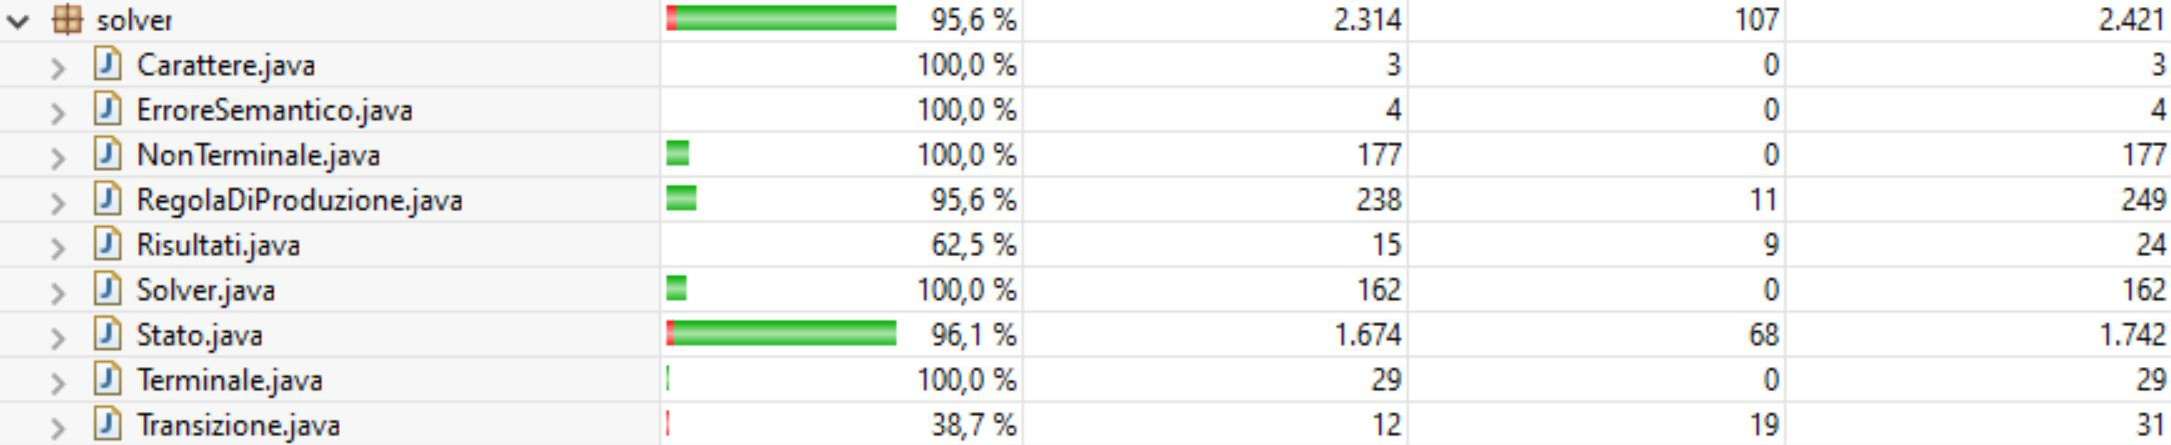
\includegraphics[width=\textwidth]{immagini/SolverCoverage.png}
\caption{Copertura dei test per il package solver}
\end{figure}
\subsubsubsection{Esiti dei test per la classe Stato}
Per la classe Stato sono stati scritti, all'interno della classe StatoTest, 22 test, superati correttamente dal programma, che garantiscono una copertura della classe Stato pari al $96,1\%$.
\begin{figure}[h]
\centering
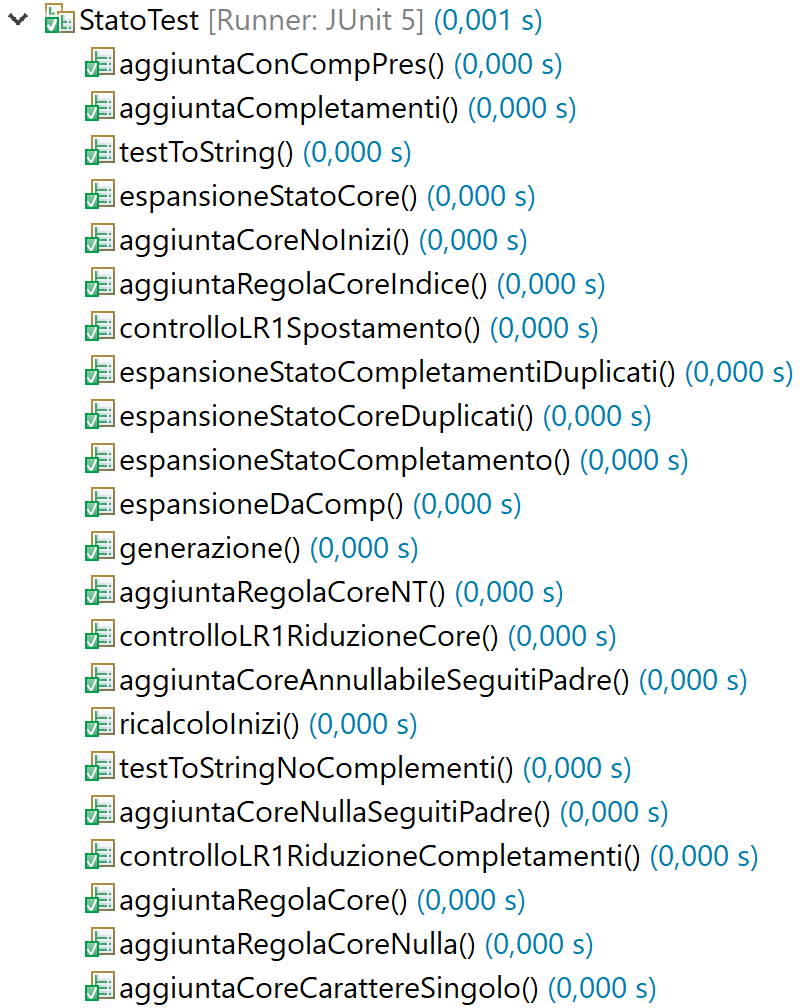
\includegraphics[scale=0.4]{immagini/esitiStatoTest.png}
\caption{Esiti dei test della classe Stato}
\end{figure}
\subsubsubsection{Esiti dei test per la classe RegolaDiProduzione}
Per la classe RegolaDiProduzione sono stati scritti, all'interno della classe RegolaDiProduzioneTest, 6 test, superati correttamente dal programma, che garantiscono una copertura della classe RegolaDiProduzione pari al $95,6\%$.
\begin{figure}[h]
\centering
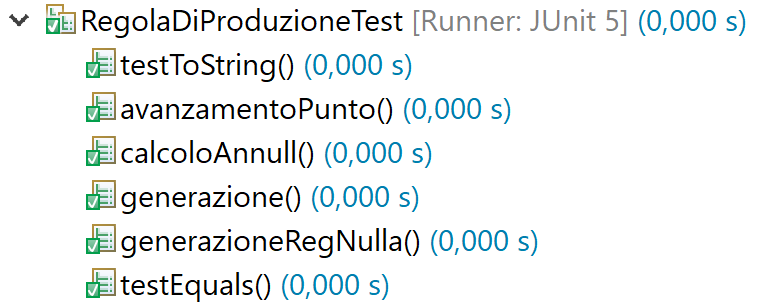
\includegraphics[scale=0.4]{immagini/esitiRegolaDiProduzioneTest.png}
\caption{Esiti dei test della classe RegolaDiProduzione}
\end{figure}
\subsubsubsection{Esiti dei test per la classe NonTerminale}
Per la classe NonTerminale sono stati scritti, all'interno della classe NonTerminaleTest, 13 test, superati correttamente dal programma, che garantiscono una copertura della classe NonTerminale pari al $100,0\%$.
\begin{figure}[h]
\centering
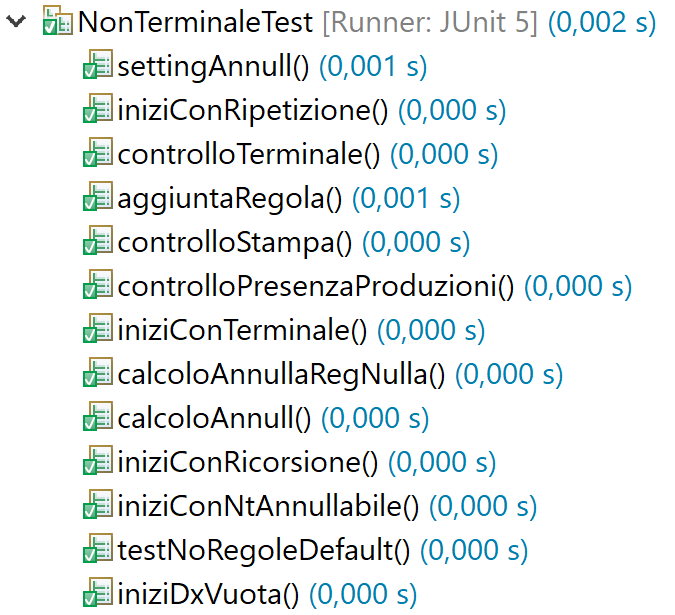
\includegraphics[scale=0.4]{immagini/esitiNonTerminaleTest.png}
\caption{Esiti dei test della classe NonTerminale}
\end{figure}
\pagebreak
\subsubsubsection{Esiti dei test per la classe Solver}
Per la classe Solver sono stati scritti, all'interno della classe SolverTest, 2 test, superati correttamente dal programma, che garantiscono una copertura della classe Solver pari al $100,0\%$.
\begin{figure}[h]
\centering
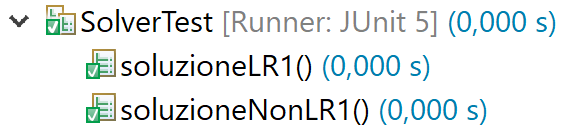
\includegraphics[scale=0.4]{immagini/esitiSolverTest.png}
\caption{Esiti dei test della classe Solver}
\end{figure}
\subsubsubsection{Esiti dei test per la classe Terminale}
Per la classe Terminale sono stati scritti, all'interno della classe TerminaleTest, 7 test, superati correttamente dal programma, che garantiscono una copertura della classe Terminale pari al $100,0\%$.
\begin{figure}[h]
\centering
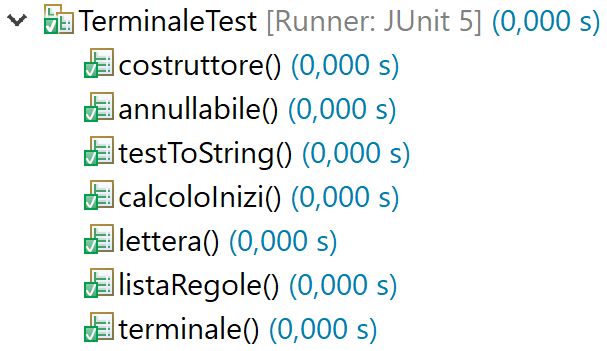
\includegraphics[scale=0.4]{immagini/esitiTerminaleTest.png}
\caption{Esiti dei test della classe Terminale}
\end{figure}
\pagebreak
\subsubsection{Esiti e copertura dei test di sistema}
I test di sistema è stato effettuato eseguendo il metodo \textit{main} della classe \textit{app}, passandogli come input i file contenuti all'interno della cartella "lfc$\backslash$resources" presente nella repository del progetto (\url{https://github.com/d-presciani/progettoLFC}); come oracoli per valutare la correttezza dei test sono stati utilizzati i temi svolti in classe durante il corso di Linguaggi formali e compilatori. \par
Durante il test di sistema è stata rilevata anche la copertura del codice durante l'esecuzione; nella seguente immagine è possibile vedere la copertura complessiva.
\begin{figure}[h]
\centering
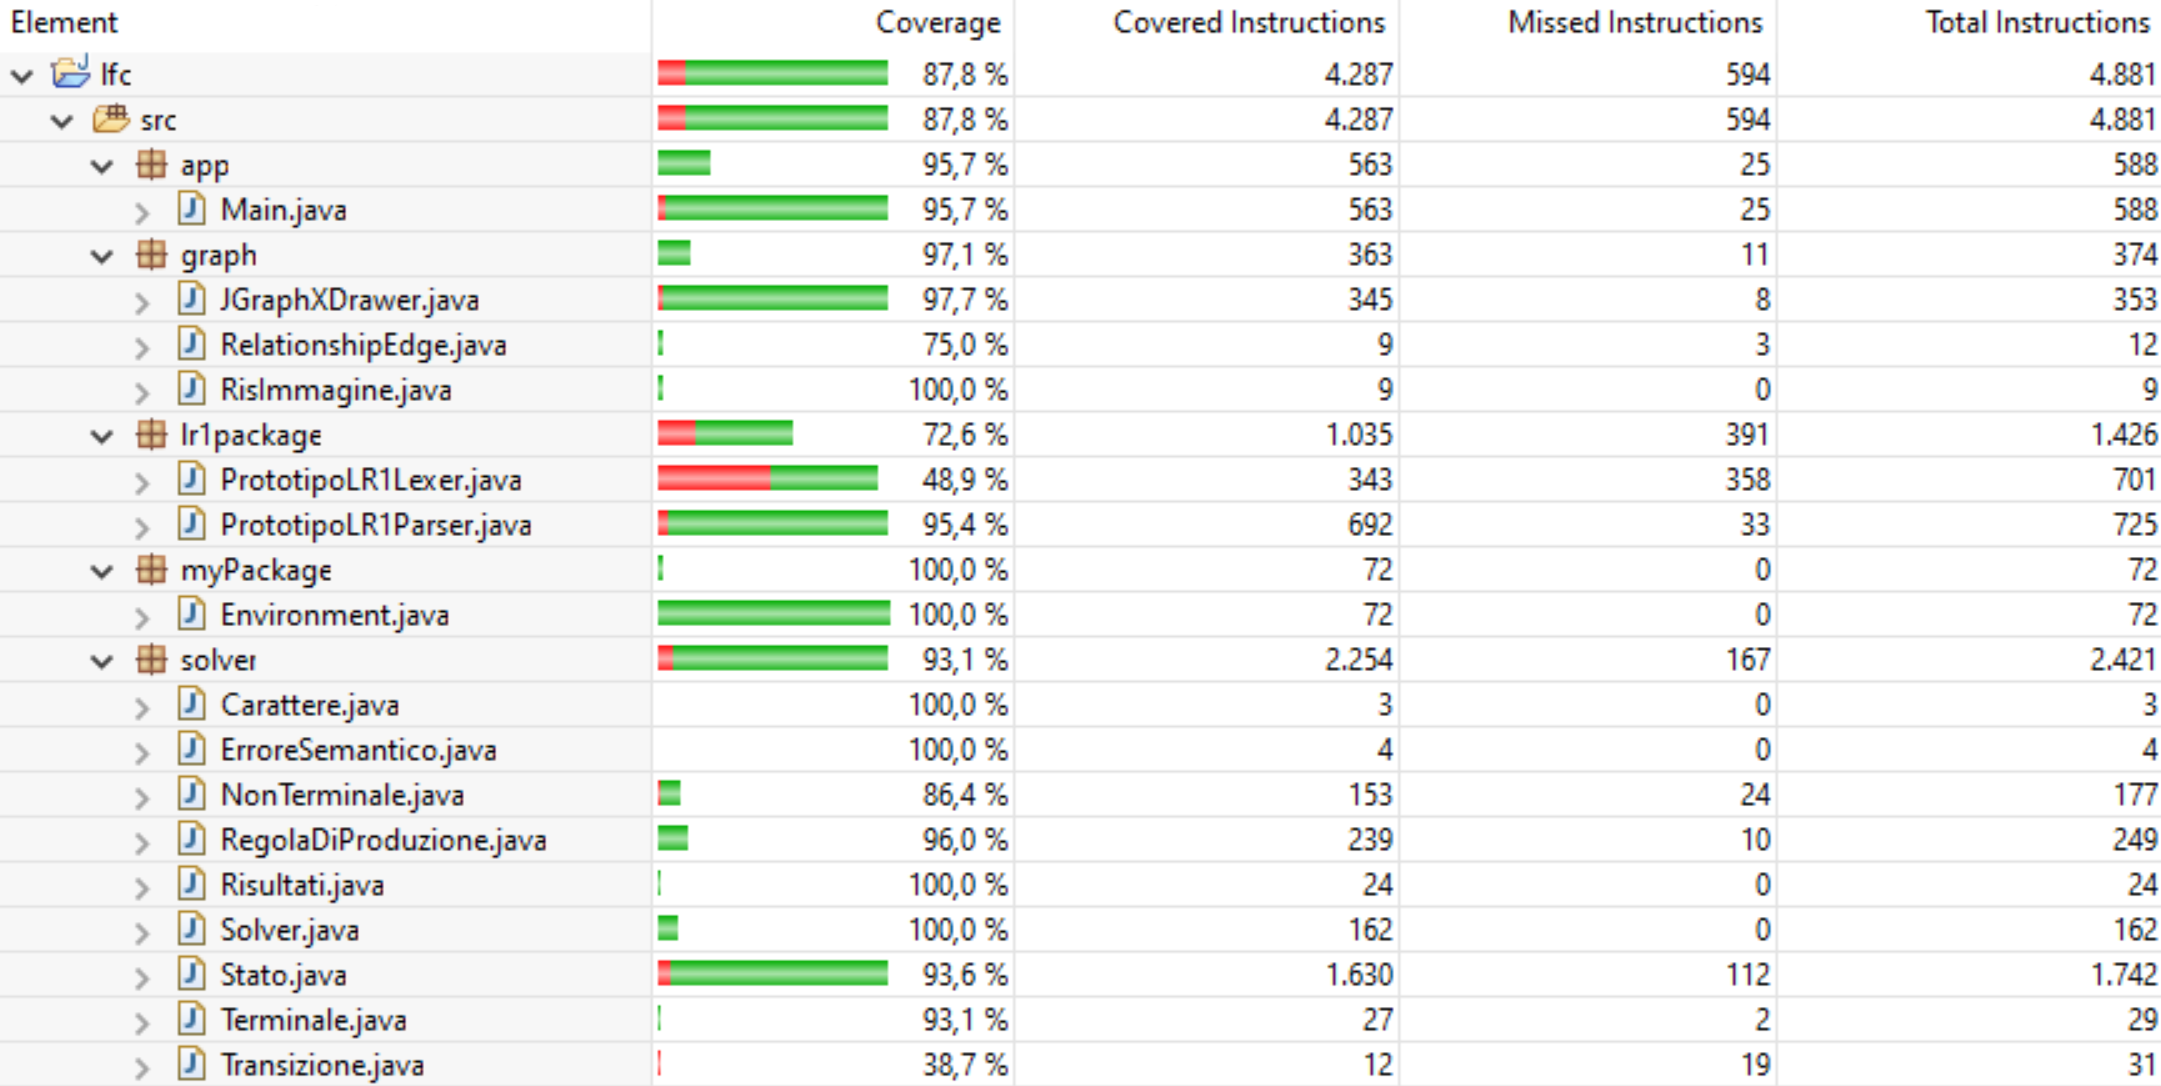
\includegraphics[width=\textwidth]{immagini/coverage.png}
\caption{Copertura del codice relativa al test di sistema}
\end{figure}
\pagebreak
\section{Sviluppi futuri}
Il programma, allo stato attuale, potrebbe essere migliorato sia sotto l'aspetto dell'interfaccia grafica che delle funzionalità, ad esempio:
\begin{itemize}
\item espandere le capacità di analisi implementando dei moduli in grado di riconoscere altri tipi di grammatiche come LALR(1) e LL(1);
\item aggiungere la possibilità di scrittura della grammatica direttamente nel programma, senza l'utilizzo di un file txt, in modo da evidenziare anche nella grammatica le regole problematiche;
\item migrazione della generazione del grafo a librerie compatibili con JavaFX al fine di avere un grafo editabile;
\item porting dell'applicazione anche per dispositivi mobili.
\end{itemize}

\end{document}